\section{What is the role of matrix size?}
In Chapter~\ref{Method} two different functions were proposed to model the relationship between grain size, number of cores, and performance (execution time or throughput). These functions were fitted for each matrix size individually for simplification, but this assumption is not practical, since even though the characteristics of the function is the same for all matrix sizes, the fitted parameters vary from one matrix size to another. 

The matrix size should somehow be integrated into the model itself. For this purpose, first we need to understand how changing the matrix size affects the relationship between grain size and performance. 
One immediate effect of increasing the matrix size is an increase in maximum possible grain size (right hand side of Figure~\ref{fig19} ) , while the minimum possible grain size is the same.

\vspace{\baselineskip}	
\begin{figure}[H]	
	\centering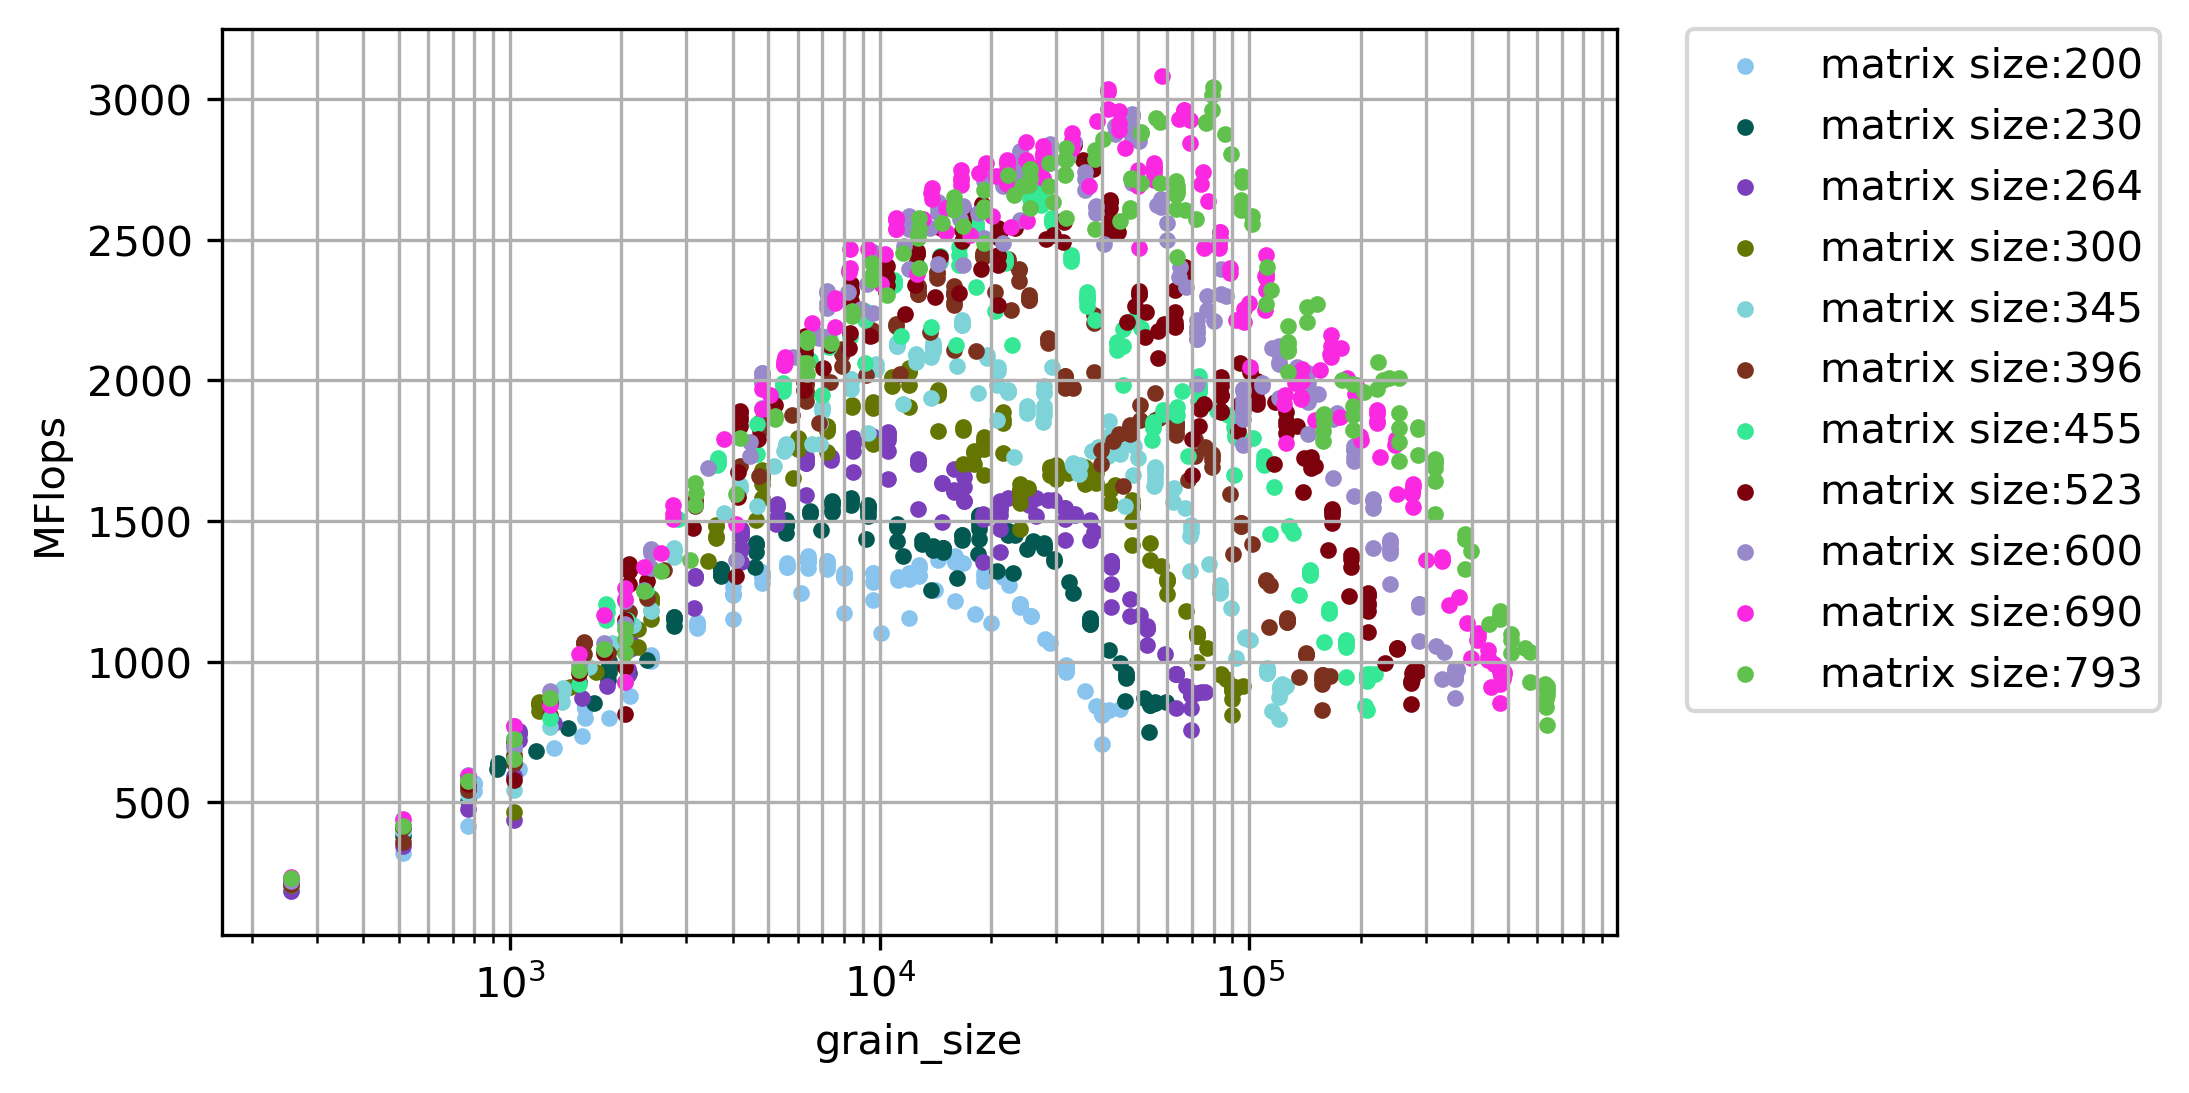
\includegraphics[scale=.75]{images/fig11.png}			
	\caption{Throughput vs. grain size graph obtained from running $DMATDMATADD$ benchmark  on $4$ cores.}
	\label{fig19}	
\end{figure} 


Moreover, Figure~\ref{fig20} shows how the predicted grain size range changes for different matrix sizes.
 
\vspace{\baselineskip}	
\begin{figure}[H]	
	\centering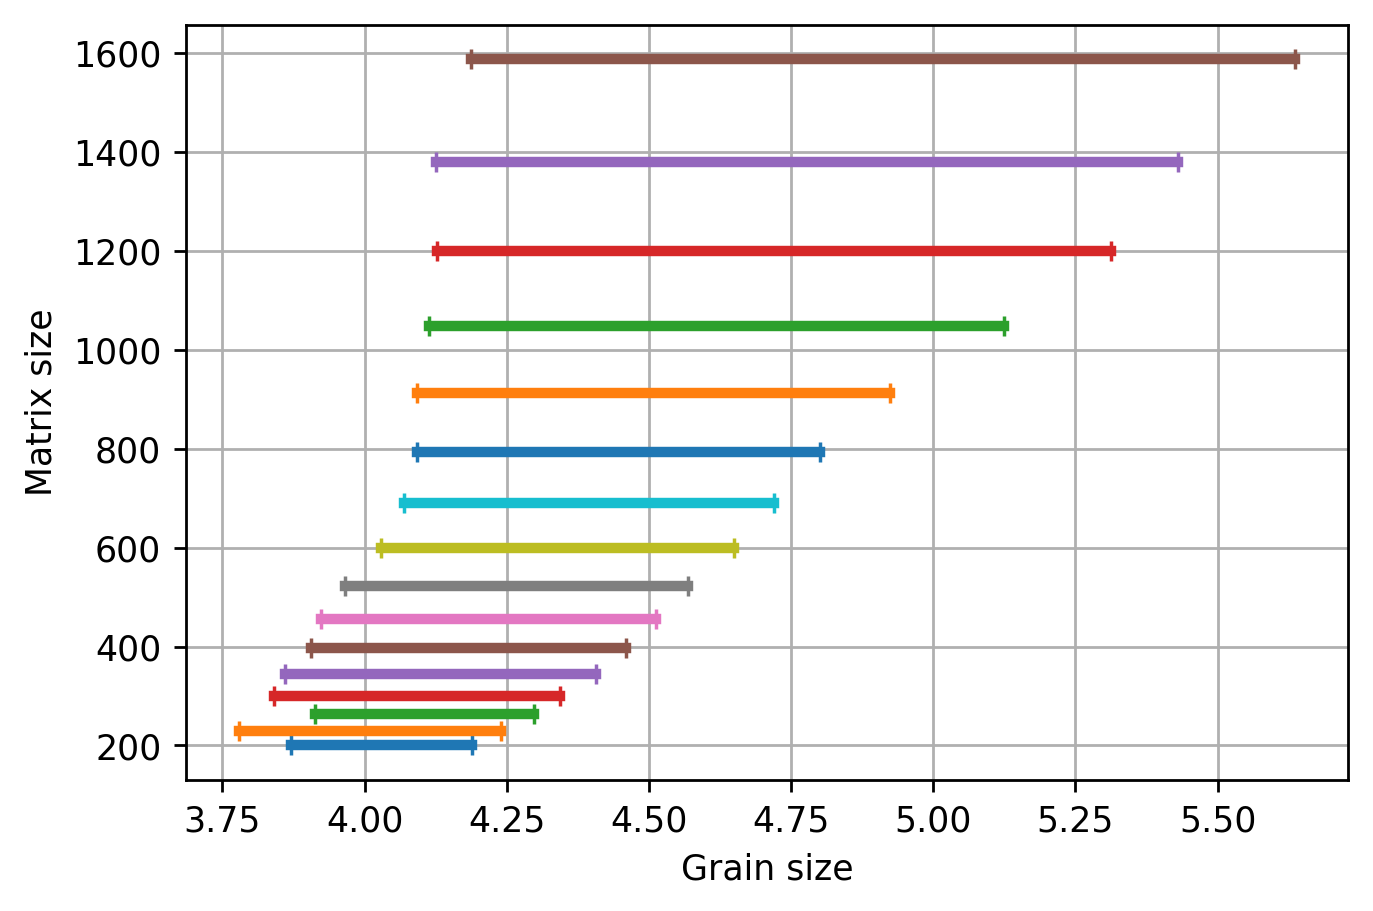
\includegraphics[scale=.75]{images/polyfit/fig_all_sizes_range_silver.png}			
	\caption{The predicted range of grain size for maximum performance for different matrix sizes, using polynomial fit, based on $DMATDMATADD$ benchmark.}
	\label{fig20}	
\end{figure} 